\renewcommand*{\arraystretch}{1.5}
\noindent\begin{tabularx}{17cm}{|p{1.95cm}|X|}
	\hline
	number      & 7                                                          \\ \hline
	title       & Most authoritative users on a given topic                                                           \\ \hline
	\multicolumn{2}{|c|}{ 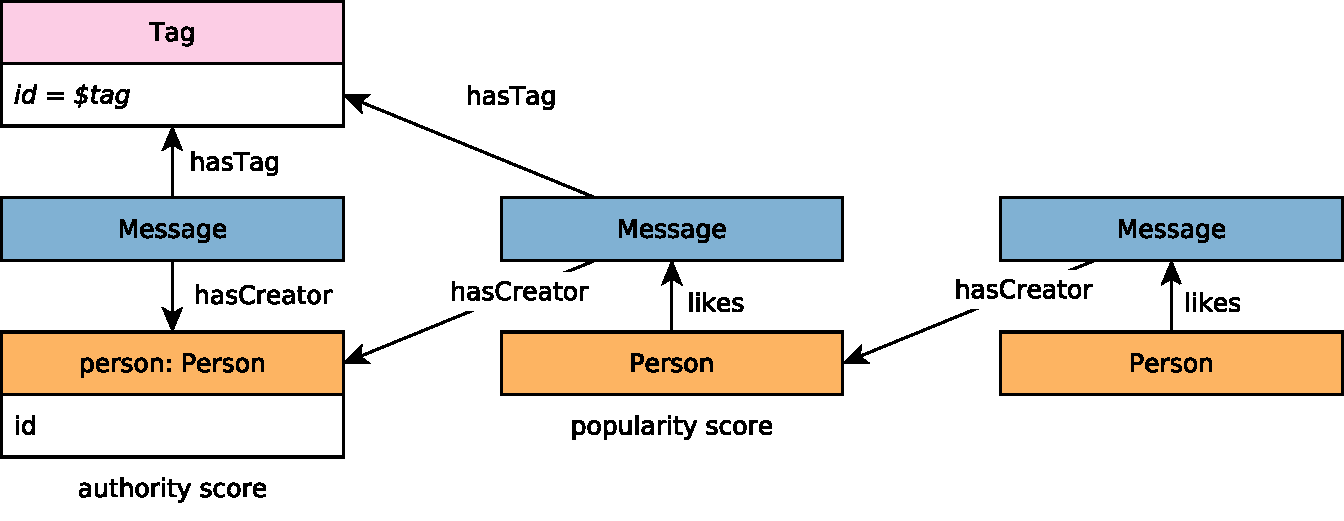
\includegraphics[scale=\patternscale,margin=0cm .2cm]{patterns/q07}} \\ \hline
	description & Given a Tag, find all Persons that ever created a Message with the given
Tag. For each of these Persons compute their ``authority score'' as
follows:

\begin{itemize}
\tightlist
\item
  The ``authority score'' is the sum of ``popularity scores'' of the
  Persons that liked any of that Person's Messages with the given Tag.
\item
  A Person's ``popularity score'' is defined as the total number of
  likes on all of their Messages.
\end{itemize}
 \\ \hline
	
	parameters  &
	\renewcommand*{\arraystretch}{1.0}
	\vspace{-1.8ex}{\begin{tabularx}{14.2cm}{|c|l|p{2cm}|Y|} \hline
	\cellcolor{black!70} \color{white} $\mathsf{1}$ & \varname{tag} & \cellcolor{gray!20} \vartype{32bitInteger} & \\ 
	\end{tabularx}} \\ \hline
	result      &
	\renewcommand*{\arraystretch}{1.0}
	\vspace{-1.8ex}{\begin{tabularx}{14.2cm}{|c|l|p{2cm}|Y|} \hline
	\cellcolor{black!70} \color{white} $\mathsf{1}$ & \varname{person1.id} & \cellcolor{gray!20} \vartype{64bitInteger} & \\ \hline
	\cellcolor{black!70} \color{white} $\mathsf{2}$ & \varname{authorityScore} & \cellcolor{gray!20} \vartype{32bitInteger} & \\ 
	\end{tabularx}} \\ \hline
	sort        &
	\renewcommand*{\arraystretch}{1.0}
	\vspace{-1.8ex}{\begin{tabular}{|c|l|c|} \hline
	\cellcolor{black!70} \color{white} $\mathsf{1}$ & \varname{authorityScore} & \cellcolor{gray!20} $\desc$ \\ \hline
	\cellcolor{black!70} \color{white} $\mathsf{2}$ & \varname{person1.id} & \cellcolor{gray!20} $\asc$ \\ 
	\end{tabular}} \\ \hline
	limit       & 100                                                           \\ \hline
	choke points        &
	\multicolumn{1}{>{\raggedright}X|}{
		\chokepoint{1.2}, 
		\chokepoint{2.3}, 
		\chokepoint{3.2}, 
		\chokepoint{3.3}, 
		\chokepoint{6.1}
		}\\ \hline
\end{tabularx}
\clearpage